\documentclass[]{beamer}
\mode<presentation>
{
    \usetheme{Warsaw}
    \definecolor{mcgarnet}{rgb}{0.38, 0, 0.08}
    \definecolor{mcgray}{rgb}{0.6, 0.6, 0.6}
    \setbeamercolor{structure}{fg=mcgarnet,bg=mcgray}
    %\setbeamercovered{transparent}
}


\usepackage[english]{babel}
\usepackage[latin1]{inputenc}
\usepackage{times}
\usepackage[T1]{fontenc}
\usepackage{tikz}
\usepackage{graphicx}
\usepackage{adjustbox}
\usepackage{fancyvrb}

\newcommand{\imagesource}[1]{{\centering\hfill\break\hbox{\scriptsize Image Source:\thinspace{\small\itshape #1}}\par}}

\title{06 - Making Decisions - Part 2}


\author{Dr. Robert Lowe\\}

\institute[Maryville College] % (optional, but mostly needed)
{
    Division of Mathematics and Computer Science\\
    Maryville College
}

\date[]{}
\subject{}

\pgfdeclareimage[height=0.5cm]{university-logo}{images/Maryville-College}
\logo{\pgfuseimage{university-logo}}



\AtBeginSection[]
{
  \begin{frame}<beamer>{Outline}
    \tableofcontents[currentsection]
  \end{frame}
}


\begin{document}

\begin{frame}
  \titlepage
\end{frame}

\begin{frame}{Outline}
  \tableofcontents
\end{frame}


% Structuring a talk is a difficult task and the following structure
% may not be suitable. Here are some rules that apply for this
% solution: 

% - Exactly two or three sections (other than the summary).
% - At *most* three subsections per section.
% - Talk about 30s to 2min per frame. So there should be between about
%   15 and 30 frames, all told.

% - A conference audience is likely to know very little of what you
%   are going to talk about. So *simplify*!
% - In a 20min talk, getting the main ideas across is hard
%   enough. Leave out details, even if it means being less precise than
%   you think necessary.
% - If you omit details that are vital to the proof/implementation,
%   just say so once. Everybody will be happy with that.

\section{Some General Advice}

\begin{frame}{Git Work Sessions}
  \begin{itemize}[<+->]
      \item Always begin each work session with:
        \newline\texttt{git pull}
      \item Frequently commit!
        \newline\texttt{git add -A}
        \newline\texttt{git commit -a}
      \item When you do a commit, git will open nano for you to
        edit your messages.  You can avoid opening the editor by
        using the \texttt{-m} option to specify a log message
        directly on the command line:
        \newline\texttt{git commit -a -m 'log message here'}
      \item Always make sure to commit and then push all changes
        at the end of a work session.
        \newline\texttt{git push}
  \end{itemize}
\end{frame}

\begin{frame}{Programming Affirmations}
  \begin{itemize}[<+->]
      \item Do not be afraid to fail.
      \item Fail quickly, fail often.
      \item You are not the one who is behind. Pretty much everyone
        in this room feels like they are the only one who hasn't caught
        on.
      \item You are doing far better than you realize. Learning to code
        is not easy.  That you are still hear means you can do this!
      \item Programming is a repeated effort. It is full of false starts
        and scrapped efforts.
      \item If you are stuck, more code is rarely the answer.  Instead
        go back to your design notes and try to find what you missed.
      \item Seeing a program through from beginning to end without 
        backtracking and reworking almost never happens.
  \end{itemize}
\end{frame}

\begin{frame}{Working With the Compiler}
    \begin{itemize}[<+>]
        \item The compiler generates two kinds of messages (warnings and errors).
        \item A \textbf{warning} is something that can indicate code that is suspected 
          to be faulty.
        \item When the compiler issues a warning, it still compiles the program.
        \item An \textbf{error} is something that means the compiler cannot
          follow the meaning of the code.  (Malformed syntax, invalid keywords, wrong types, etc.)
        \item When an error occurs, the compiler does not generate code.
    \end{itemize}
\end{frame}

\begin{frame}[fragile]{Locating Errors}
  \begin{BVerbatim}
even-odd.cpp: In function 'int main()':
even-odd.cpp:19:5: error: expected ';' before '}' token
     } else {
     ^
  \end{BVerbatim}
  \begin{itemize}[<+->]
    \item Compiler error messages will indicate where the error/warning was located.
    \item The format is \texttt{filename}:\textit{line}:\textit{column}
    \item The above error is from file \texttt{even-odd.cpp} line 19 column 5
    \item The location is where the problem was noticed.  Not necessarily where
      it actually needs to be fixed.
    \item Compilers do nothing to detect logic errors!
  \end{itemize}
\end{frame}

\begin{frame}{Challenge: Fix \texttt{proportion.cpp}}
  \begin{enumerate}[<+->]
      \item Make the directory \texttt{labs/week4}
      \item Copy the file \texttt{examples/06-Decisions/proportion.cpp} to your \texttt{labs/week4} directory.
      \item Try to compile \texttt{proportion.cpp}. 
      \item Use the compiler error messages to locate and fix the compiler errors. 
      \item Test the program.  Fix any logic errors you may find.
  \end{enumerate}
\end{frame}

\begin{frame}{UNIX Tips and Shortcuts}
    \begin{itemize}[<+->]
        \item Typing part of a filename followed by the \texttt{tab} key will complete the filename for you.
        \item You can scroll through your command history by pressing up and down on the cursor keys.
        \item Repeat a selected command by pressing \texttt{enter}.
        \item You can repeat a command by pattern matching using \texttt{!}.  For example, to repeat your last compiler line:
          \newline\texttt{!g++}
          \newline or
          \newline\texttt{!g}
        \item Try using these as you use the command line.  More speed tips will follow.
    \end{itemize}
\end{frame}


\section{Advanced Decision Making}


\begin{frame}[fragile]{Testing for a Range of Values}
  \begin{itemize}[<+->]
    \item In your \texttt{examples/06-Decisions} folder, you will find \texttt{range.cpp}
    \item Run and test this program.  Does it work?
    \item What is going on here?
  \end{itemize}
  \begin{adjustbox}{max height=4.75cm}
  \begin{BVerbatim}
int main()
{
    int num;

    //get a number
    cout << "Enter a number" << endl;
    cin >> num;

    //test to see if it is between 1 and 5
    if(1 <= num <= 5) {
        cout << "The number is between 1 and 5" << endl;
    } else {
        cout << "The number is not between 1 and 5" << endl;
    }
}
  \end{BVerbatim}
  \end{adjustbox}
\end{frame}

\begin{frame}{Combinational Operators}
  \begin{columns}
    \column{0.3\textwidth}
    \begin{center}
        \texttt{\textbf{and}}
        \newline\newline
        \begin{tabular}{cc|c}
          \texttt{a} & \texttt{b} & \texttt{a and b} \\
          \hline
          F & F & F\\
          F & T & F\\
          T & F & F\\
          T & T & T\\
        \end{tabular}
    \end{center}

    \column{0.3\textwidth}
    \begin{center}
        \texttt{\textbf{or}}
        \newline\newline
        \begin{tabular}{cc|c}
          \texttt{a} & \texttt{b} & \texttt{a or b} \\
          \hline
          F & F & F\\
          F & T & T\\
          T & F & T\\
          T & T & T\\
        \end{tabular}
    \end{center}

    \column{0.3\textwidth}
    \begin{center}
        \texttt{\textbf{not}}
        \newline\newline
        \begin{tabular}{c|c}
          \texttt{a} & \texttt{not a} \\
          \hline
          F & T \\
          T & F \\
        \end{tabular}
    \end{center}
  \end{columns}
\end{frame}

\begin{frame}{Operator Precedence (Thus Far)}
    \begin{tabular}{|l|l|l|}
        \hline
        \textbf{Operator} & \textbf{Description} & \textbf{Associativity} \\
        \hline
        \texttt{not}, \texttt{!} & Logical Not & Left-to-Right\\
        \hline
        \texttt{a*b}, \texttt{a/b}, \texttt{a\%b} & Multiply, Divide, Modulus & Left-to-Right\\
        \hline
        \texttt{a+b}, \texttt{a-b} & Addition and Subtraction & Left-to-Right\\
        \hline
        \texttt{<<} , \texttt{>>} & Insertion and Extraction & Left-to-Right \\
        \hline
        \texttt{<}, \texttt{<=} & Relational Operators & Left-to-Right\\
        \texttt{>}, \texttt{>=} & & \\
        \hline
        \texttt{==}, \texttt{!=} & Equality Operators & Left-to-Right\\
        \hline
        \texttt{and}, \texttt{\&\&} & Logical And & Left-to-Right\\
        \hline
        \texttt{or}, \texttt{||} & Logical Or & Left-to-Right\\
        \hline
        \texttt{=},  & Assignment and Assignment & Right-to-Left \\
        \texttt{+=}, \texttt{-=} & & \\
        \texttt{*=}, \texttt{/=} & & \\
        \texttt{\%=} & & \\
        \hline
    \end{tabular}
\end{frame}


\begin{frame}{Example: Range Validate}
  \begin{center}
      \texttt{num >= 1 and num <= 5}
  \end{center}
  \begin{itemize}[<+->]
      \item The above expression is the correct way to detect over a range.
      \item Copy \texttt{range.cpp} to your \texttt{labs/week4} folder and correct it.
      \item Make sure the program works!
  \end{itemize}
\end{frame}

\begin{frame}[fragile]{Multi-Way Branching: If-Then-Else-If}
\begin{columns}
    \column{0.5\textwidth}
    \verb!if(! \textit{condition} \verb!)! 
    \newline\verb!    ! \textit{then statement/block}
    \verb!else if(! \textit{condition} \verb!)! 
    \newline\verb!    ! \textit{then statement/block}
    \newline\verb!else!
    \newline\verb!    ! \textit{else statement/block}
    
    \vspace{0.5cm}

    \begin{itemize}[<+(1)->]
        \item The first then \textit{statement/block} with a true condition executes.
        \item If no matches are found, the (optional) \textit{else statement/block} executes.
    \end{itemize}

    \column{0.5\textwidth}
    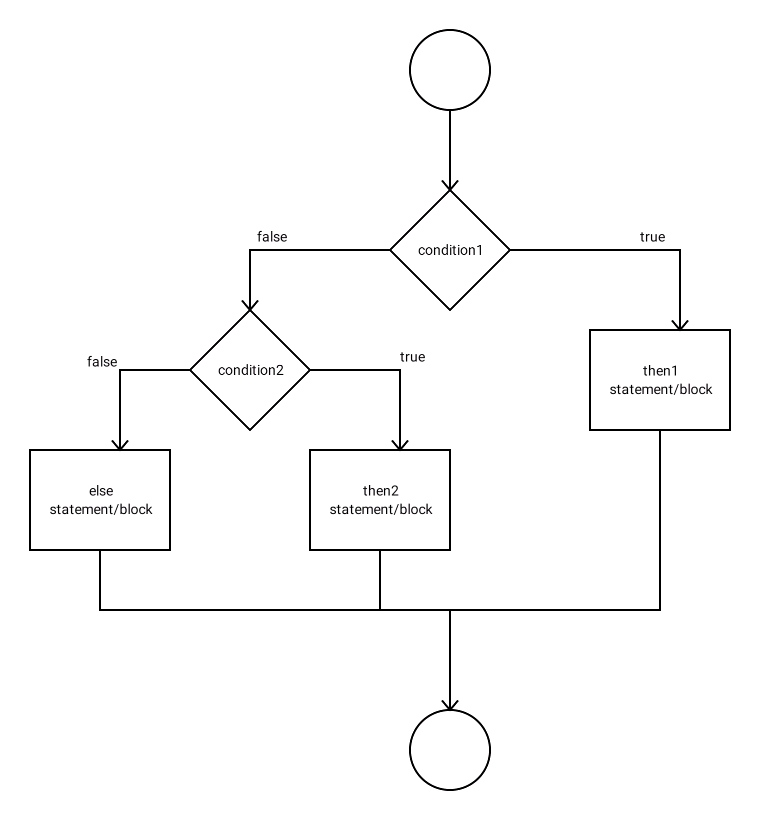
\includegraphics[width=0.9\textwidth]{images/if-elseif}
\end{columns}
\end{frame}

\begin{frame}[fragile]{Example Snippet: Rock, Paper Scissors}
  \begin{BVerbatim}
  if(player == 1) {
    cout << "Rock" << endl;
  } else if(player == 2) {
    cout << "Paper" << endl;
  } else if(player ==3) {
    cout << "Scissors" << endl;
  }
  \end{BVerbatim}
\end{frame}

\begin{frame}[fragile]{Challenge: The Stock Menu}
  \begin{adjustbox}{max height=0.45\textheight}
  \begin{BVerbatim}
        Stock Portfolio Management System
                Please Make a Selection
        1 -- Buy a Stock
        2 -- Sell a Stock
        3 -- Report Current Holdings
        4 -- Report Gains and Losses
        5 -- Remove a Current Holding
        6 -- Done!  (quit) 

        Choice? 
  \end{BVerbatim}
  \end{adjustbox}
  \begin{enumerate}[<+(1)->]
    \item Copy your \texttt{stock.cpp} file from your \texttt{labs/week2} directory to your \texttt{labs/week4} directory.
    \item Add logic so that it prints your menu selection.  For instance, if you enter ``1'', your program should reply with ``\texttt{Buy a Stock}''
    \item Add logic so that if you select anything other than 1 through 6, your program displays an error message.
  \end{enumerate}
\end{frame}

\end{document}


